% Section 1 - Services
% Roberto Masocco <roberto.masocco@uniroma2.it>
% April 21, 2022

% ### Services ###
\section{Services}
\graphicspath{{figs/section1/}}

% --- ROS 2 Services ---
\begin{frame}{ROS 2 Services}
ROS 2 extends the basic DDS messages adding two more communication paradigms: the first is the \textbg{service}. It allows nodes to establish \textbg{client-server} communications.
\begin{figure}
  \centering
  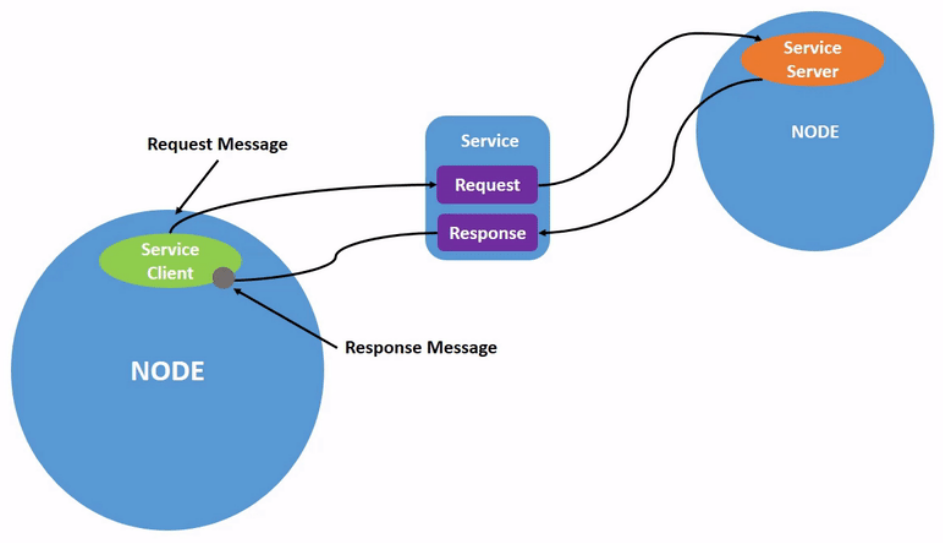
\includegraphics[scale=.35]{ros2Srv.png}
  \label{fig:ros2srv}
  \caption{Two nodes acting as service \emph{client} and \emph{server}}
\end{figure}
\end{frame}
\begin{frame}{ROS 2 Services}
In actual ROS 2 applications:
\begin{enumerate}
  \item The \textbg{client} sends a \textbg{request message} to the server.
  \item The \textbg{server} receives the request and processes it.
  \item Meanwhile, the \textbg{client} can either \textbg{block} waiting for the response or \textbg{synchronously poll} it.
  \item When done, the \textbg{server} sends a \textbg{response message} to the client.
  \item If waiting, the \textbg{client} awakes when receiving the reponse.
\end{enumerate}
\end{frame}

% --- Coding Servers and Clients ---
\begin{frame}{Coding Servers and Clients}
  \begin{block}{Servers}
    Similarly to topic subscriptions, requests are processed in appropriate \textbf{callbacks}, in which responses are also populated. The server object is as well only needed to instantiate the service.
  \end{block}
  \begin{block}{Clients}
    As per the previous dynamics, one has to \textbf{code each step} of the client side into their application using appropriate \textbf{ROS 2 APIs}. The client object is used to send requests, while \textbf{responses are handled as \texttt{future} objects\footnote{\href{https://en.cppreference.com/w/cpp/thread/future}{\color{blue}\underline{\texttt{std::future} - C++ Reference}}}} (related to \emph{asynchronous I/O}, no further details required).
  \end{block}
\end{frame}

% --- Interface Files - Services ---
\begin{frame}[fragile]{Interface Files - Services}
The entire system is built on messages, so \textbg{combine two of them} in a single interface file, separated by \texttt{-{}-{}-}.\\
Service file names end with \texttt{.srv}.
\begin{columns}
\column{.9\textwidth}
% Listing: example_interfaces/srv/AddTwoInts service definition
\begin{lstlisting}[language=ros2msg, caption=Definition of the \texttt{example\_interfaces/srv/AddTwoInts} service]
# REQUEST
int64 a
int64 b
---
# RESPONSE
int64 sum
\end{lstlisting}
\end{columns}
\end{frame}

% --- Example: Simple Service ---
\begin{frame}{Example: Simple Service}
Now go have a look at the \href{https://github.com/IntelligentSystemsLabUTV/ros2-examples/tree/galactic/src/simple_service}{\color{blue}\underline{ros2-examples/src/simple\_service}} package!
\end{frame}
